\scanpage{48}
\mspage{\handwritten{19}}

\begingroup
\setbox0=\vbox{%
  \hsize=\linewidth
  \parindent=0pt
  \parskip=.7\baselineskip
  9.1.13. \uline{Questions ouvertes}. Soit $E$ un \uline{U}-topos.\par

  a) Dans l'ensemble
  \mbox{\rlap{\raise2.1ex\hbox{\inserted{ordonné}}}%
    \rlap{\begin{tikzpicture}[overlay,baseline=0pt,x=1em,y=1ex,line cap=round]
      \draw[line width=.45pt] (-.2,-.35) .. controls (.05,1.35) and (.2,1.55) .. (.55,1.55)
        -- (4.6,1.55) .. controls (4.9,1.55) and (5,1.8) .. (4.95,2.05);
    \end{tikzpicture}}des}
  sous-topos de, $E$, le Inf de deux éléments est-il distributif par rapport \mbox{\rlap{\begin{tikzpicture}[overlay,baseline=0pt,x=1em,y=1ex,line cap=round]
    \draw[line width=.5pt] (.48,-.05) .. controls (.55,-.25) and (.65,-.45) .. (.78,-.48);
  \end{tikzpicture}}aux} Sup finis ? Pour des résultats dans c e \deleted{\unsure{se}} sens, voir 9.1.11 e) et 9.1.12 d) .\par

  b) Soit $E'$ un sous-topos de $E$, distinct \unsure{de|du} \deleted{sous-topos ``vide''} $E$. Existe-t-il un sous-topos $E''$ de $E$, tel que $E''\handwritten{\cap}E'=\operatorname{Top}(\varnothing)$, $E''\handwritten{\ne}\operatorname{Top}(\varnothing)$ ?\par

  c\deleted{p}) Soient $E'$ et $E''$ deux sous-topos de $E$ tels que $E'\handwritten{\cap}E''=\operatorname{Top}(\varnothing)$. Les conditions suivantes sont-elles équivalentes: (i) $E$ est le sup de $E'$ et $E''$ dans l'ensemble des sous-topos de $E$ (on se retient à grand peine d'écrire cette condition $E=E'\handwritten{\deleted{\unsure{\cap|\vee}}\cup}E''$ ); (ii) $E''$ est \unsure{\deleted{m}ax|\deleted{max}} \unsure{la|le} plus grand parmi les sous-topos $E''_{1}$ de $E$ tels que $\operatorname{Top}(E')\handwritten{\cap}\operatorname{Top}(E''_{1})=\operatorname{Top}(\varnothing)$; (iii) $E''$ est maximal parmi les $E''_{1}$ précédents.\par

  \noindent\rlap{%
    \begin{tikzpicture}[overlay,baseline=0pt,x=1em,y=1ex,line cap=round,line join=round]
      \draw[black!25,line width=.35pt] (-1.15,.05) -- (-1.05,3.1) -- (.2,2.55);
      \draw[black!25,line width=.35pt] (-.2,2.15) -- (-.65,1.75) -- (-.05,1.5)
        -- (-.65,.85) -- (-.1,.45) -- (-.4,-.15);
      \draw[line width=.85pt] (-1.8,-.6) .. controls (-1.3,-.45) and (-.7,-.65) .. (-.15,-.6)
        .. controls (-.3,.3) and (-.32,1.1) .. (-.38,1.9);
      \draw[line width=.85pt] (-.34,1.35) -- (-.17,1.82);
      \draw[line width=.85pt] (-.5,2.25) .. controls (-.05,2.4) and (.5,2.1) .. (.98,2.28);
    \end{tikzpicture}}%
  Il est \deleted{a bit} clair que (ii)$\handwritten{\Longrightarrow}$(iii), que si a) est vérifié \unsure{on|en} a (i)$\handwritten{\Longrightarrow}$(ii), \deleted{\unsure{eque si|e que si}} \inserted{que} b) est \unsure{vérifié|vérifi} \deleted{\unsure{é|e}} \inserted{si et seulement si \deleted{on a}} on a (iii)$\handwritten{\Longrightarrow}$(i); donc une solution affirmative à a) et b) en impliqu\unsure{e|r}rait une pour c). Noter aussi que la réponse aux questions posées \inserted{( y compris d) qui suit)} est affirmative si $E$ est de la forme $\operatorname{Top}(X)$, $X$ un espace topologique
  \mbox{\rlap{\raise2.1ex\hbox{\inserted{localement}}}%
    \rlap{\begin{tikzpicture}[overlay,baseline=0pt,x=1em,y=1ex,line cap=round]
      \draw[line width=.45pt] (-.15,-.2) .. controls (-.8,-.1) and (-.3,1.4) .. (.2,1.4)
        .. controls (2.4,1.4) and (5.9,1.4) .. (6.4,1.9)
        .. controls (6.6,2.1) and (6.6,2.3) .. (6.6,2.5);
    \end{tikzpicture}}noethérien}
  (9.1.11 b)), \deleted{ainsi que pour $E=G$} \inserted{\deleted{ou si $E$ est}} un topos fini (9.1.12).\par

  d) Si $E$ est le sup des deux sous-topos $E'$ et $E''$, alors tout point de $E$ est-il isomorphe à un point provenant de $E'$ ou de $E''$ ?\par

  Si la réponse à d) était affirmative, alors on aurait une réponse affirmative à a) \inserted{$(E'\ (E''\ E''')=E'\ E''\quad E'\ E''')$} pour le\deleted{s} cas de sous-topos $E',E'',E'''$ de $E$ ayant suffisamment de points (donc a) serait vrai pour $E$ \inserted{localement} noethérien, en vertu de 9.1.11 b)). Inversement, si a)\par
}%
\dimen0=\wd0
\dimen2=\ht0
\edef\scanblockwidth{\the\dimen0}
\edef\scanblockheight{\the\dimen2}
\noindent\hbox{%
  \rlap{\raise\ht0\hbox{%
    \begin{tikzpicture}[overlay,baseline=0pt,x=\scanblockwidth,y=-\scanblockheight,line cap=round]
      \draw[black!30,line width=.4pt] (.47,-.025) .. controls (.46,.025) and (.445,.06) .. (.43,.105);
      \draw[black!80,line width=.55pt] (.43,.105) .. controls (.385,.31) and (.345,.62) .. (.342,.975);
      \draw[black!65,line width=.45pt] (.342,.987) -- (.337,1.005);
    \end{tikzpicture}%
  }}%
  \box0
}\par
\endgroup

% archive sheet number: 47
